\documentclass{beamer}
\usetheme[sectionpage=none]{metropolis}
% Theme settings
\setbeamerfont{footnote}{size=\tiny}

\usepackage[utf8]{inputenc}
\usepackage[T1]{fontenc}
\usepackage{textcomp}
\usepackage{babel}
\usepackage{amsmath, amssymb, mathtools}
\usepackage{listings}
\usepackage[ruled,vlined]{algorithm2e}

% % figure support
\usepackage{multimedia}
\usepackage{import}
\usepackage{xifthen}
\usepackage{pdfpages}
\usepackage{tikz}
\usepackage{pgfplots}
\pgfplotsset{compat=1.16}
\usepackage{transparent}
\usepackage{subcaption}

\usepackage[backend=biber]{biblatex}
\usepackage{csquotes}
\usepackage{bm}

\addbibresource{reference.bib}

\pdfsuppresswarningpagegroup=1

\title{
  A Variety of Approaches to \\
  the Nonuniform Fast Fourier Transform
}
\author{Kosuke Sugita and Connor Robertson}
\date{December 17, 2021}

\begin{document}
\frame{\titlepage}
% \frame{\tableofcontents}

% SECTIONS
%%%%%%%%%%%%%%%%%%%%%%%%%%%%%%%%%%%%%%%%%%%%%%%%%%%%%%%%%%%%%%%%%%%%%%%%%%%%%%%
\section{Introduction}
%%%%%%%%%%%%%%%%%%%%%%%%%%%%%%%%%%%%%%%%%%%%%%%%%%%%%%%%%%%%%%%%%%%%%%%%%%%%%%%
\begin{frame}
    \frametitle{Introduction}
    \textbf{Applications for NUFFT:}
    \begin{itemize}
        \item MRI Imaging - magnetic field reads frequency domain at nonuniform points
        \item Numerical solutions to PDEs - consider radial points or Chebyshev points to better resolve domain
        \item Coarse graining particles - Nonuniform distribution of discrete items to continuous field
    \end{itemize}

    \vfill

    Nonuniform samples: $(x_n, f(x_n))$:
    \begin{align*}
        \hat{f}(k) = \sum_{n=0}^{N-1} f(x_n) e^{-i x_n k} \approx \int_{-\infty}^{\infty} f(x) e^{-i x k}dx
    ,\end{align*}
    *\textit{Order $O(N^{2})$}
\end{frame}

\begin{frame}
  \frametitle{Concept}
  \textbf{Key idea:}
  \begin{enumerate}
      \item Need uniform points for FFT symmetry
      \item Use nonuniform points to cheaply sample uniform points
  \end{enumerate}

  \vfill

  \begin{columns}
      \begin{column}{.5\textwidth}
        \textbf{Approaches:}
        \begin{itemize}
            \item Interpolation
            \item Convolution of mollifier / window function
            \item Low rank approximation to DFT matrix
        \end{itemize}
      \end{column}
      \begin{column}{.5\textwidth}
        \centering 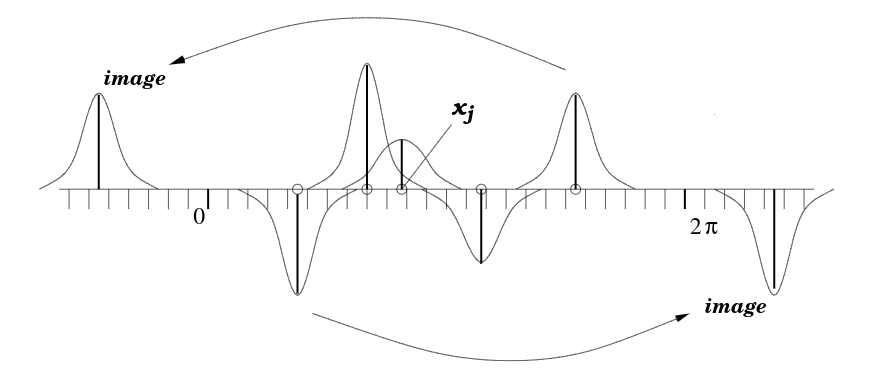
\includegraphics[width=\textwidth]{images/sample_gaussian.png}
      \end{column}
  \end{columns}
\end{frame}

\section{Numerical Examples}

\begin{frame}
  \frametitle{Sampling uniform points}
  Different sampling methods illustrated:

  \vfill

  \centering 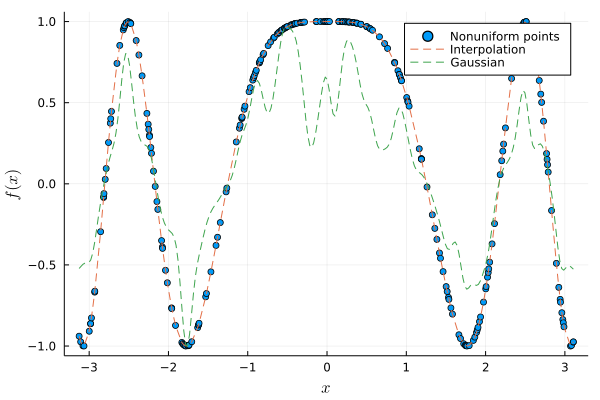
\includegraphics[width=.8\textwidth]{images/conv_vs_interp.png}
\end{frame}

\begin{frame}
  \frametitle{Comparison of methods output}
  Spectrum of results:

  \vfill

  \centering 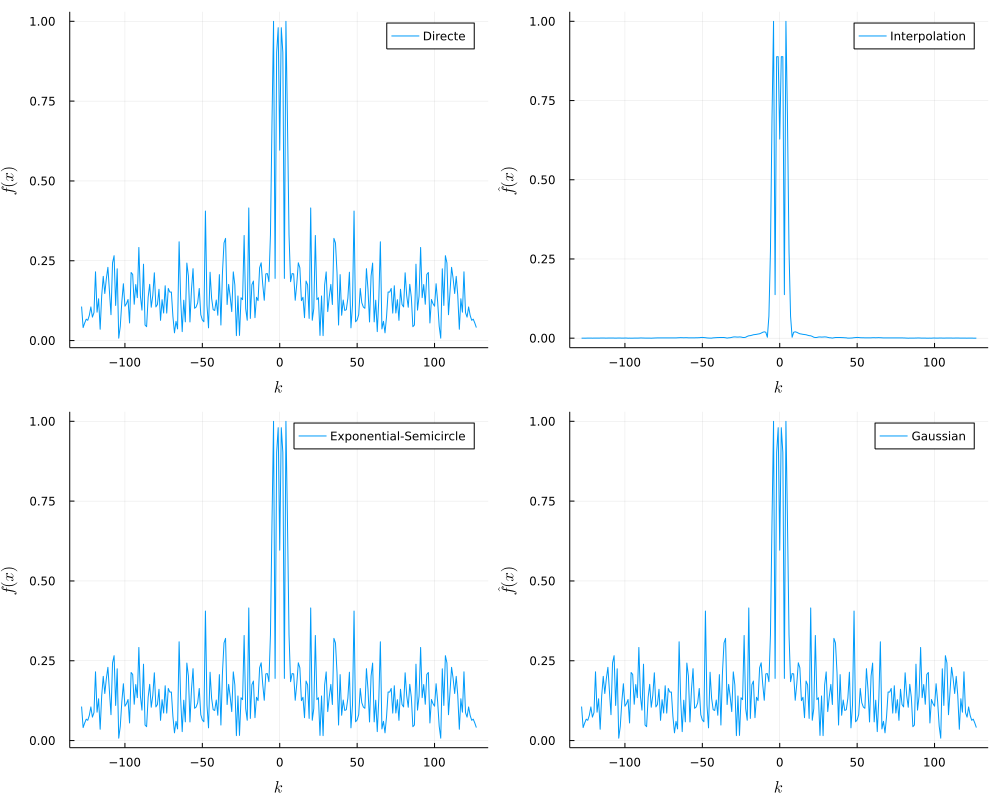
\includegraphics[width=.8\textwidth]{images/spectrum.png}

\end{frame}

%%%%%%%%%%%%%%%%%%%%%%%%%%%%%%%%%%%%%%%%%%%%%%%%%%%%%%%%%%%%%%%%%%%%%%%%%%%%%%%
\section{Numerical Methods}
%%%%%%%%%%%%%%%%%%%%%%%%%%%%%%%%%%%%%%%%%%%%%%%%%%%%%%%%%%%%%%%%%%%%%%%%%%%%%%%
\begin{frame}
    \sectionpage
\end{frame}

\begin{frame}{Type-$1$ with Gaussian Kernel}
  \begin{itemize}
    \item Input: $(f_{j})_{j=0}^{N-1}$ at nonuniform $(x_{j})_{j=0}^{N-1}$,
    \item Output: $(F_{k})_{k=0}^{M-1}$ at uniform $-M/2 \le k \le M/2-1$.
  \end{itemize}
  Assume $f(x) = \sum_{j=0}^{N-1}f_{j}\delta(x - x_{j}) \quad x \in [0,2\pi]$ and define
  \begin{align}
    g_{\tau}(x) &:= \sum_{l=-\infty}^{\infty}\exp\left(-\frac{1}{4\tau}(x-2\pi l)^2\right), \\
    f_{\tau}(x) &:= f\ast g_{\tau} (x) 
      = \int_{0}^{2\pi} f(y)g_{\tau}(x-y) dy.
  \end{align}
  $f_{\tau}$ is $C^{\infty}$ and $2\pi$-periodic (approximated by the trapezoidal rule).
\end{frame}

\begin{frame}{Type-$1$ with Gaussian Kernel}
  \begin{equation}
      f_{\tau}(2\pi\frac{m}{M_{r}}) 
    \simeq \frac{1}{N}\sum_{j=0}^{N-1} f_{j} g_{\tau}(2\pi m/M_{r} - x_{j})
  \end{equation}
  with a sufficiently large $M_{r} \in \mathbb{N}$ and $0 \le m \le M_{r}-1$. Then
  \begin{equation}
    F_{\tau}(k) = \sum_{m=0}^{M_{r}-1}f_{\tau}(2\pi m/M_{r})\exp(2\pi ikm/M_{r})
  \end{equation}
  by the uniform FFT. Finally, 
  \begin{equation}
    F(k) = \sqrt{\pi/\tau}\exp(\tau k^2)F_{\tau}(k)
  \end{equation}
  by the convolusiton theorem.
\end{frame}

\begin{frame}{Type-$2$ with Gaussian Kernel}
  \begin{itemize}
    \item Input: $(F_{k})_{k=0}^{M-1}$ at uniform $-M/2 \le k \le M/2-1$,
    \item Output: $(f_{j})_{j=0}^{N-1}$ at nonuniform $(x_{j})_{j=0}^{N-1}$.
  \end{itemize}
  Assume $f_{-\tau}$ s.t. $(f_{-\tau}\ast g_{\tau})(x) \simeq f(x)$ implying 
  $F_{-\tau}G_{\tau} \simeq F$. Then 
  \begin{equation}
      f_{-\tau}(x) 
    = \frac{1}{M_{r}}\sum_{k=0}^{M_{r}-1} F_{-\tau}(k)e^{ikx}
    = \frac{1}{M_{r}}\sum_{k=0}^{M_{r}-1} \frac{F(k)}{G_{\tau}}e^{ikx}
  \end{equation}
  is computed by the uniform inverse FFT. Then 
  \begin{align}
       f(x_{j}) 
    &\simeq f_{-\tau}\ast g_{\tau}(x_{j}) \\
    &\simeq \frac{1}{M_{r}}\sum_{m=0}^{M_{r}-1}f_{-\tau}(2\pi m/M_{r})g_{\tau}(x_{j} - 2\pi m/M_{r}).
  \end{align}
\end{frame}

\begin{frame}{Type-$3$ with Gaussian Kernel}
  Both input $(f_{j})_{j=0}^{N-1}$ and output $(F(s_{k}))_{k=0}^{M-1}$ are nonuniform.
  Type-$3$ NUFFT 
  \begin{enumerate}
    \item Split the `nonuniform-nonuniform' data processing into two steps
    by inserting the intermediate uniform data construction between.
    \item Apply Type-$1$ method to the first `nonuniform-uniform' step by convolving the input data.
    \item Apply Type-$2$ method to the second 'uniform-nonuniform' step by deconvolving the intermediate data.
  \end{enumerate}
\end{frame}

\begin{frame}{Type-$3$ with Gaussian Kernel}
  First, convolve $f$ 
  \begin{equation}
      f_{\tau}(x) = f\ast g_{\tau} (x) = \int_{0}^{2\pi} f(y)g_{\tau}(x-y) dy.
  \end{equation}
  Next, assuming $f_{\tau}^{-\sigma}$ and $F_{\tau}^{-\sigma} = \mathcal{F}[f_{\tau}^{-\sigma}]$
  s.t. 
  $f_{\tau}^{-\sigma}G_{\sigma} = f_{\tau}$ and $F_{\tau}^{-\sigma}\ast g_{\sigma} = F_{\tau}$
  with an additional parameter $\sigma$. Then 
  \begin{align}
    F_{\tau}(s) &= F_{\tau}^{-\sigma}\ast g_{\sigma} (s) \\
    &\simeq \frac{1}{M_{r}}\sum_{m=0}^{M_{r}}
            F_{\tau}^{-\sigma}(2\pi m/M_{r})g_{\sigma}(s - 2\pi m/M_{r}).
  \end{align}
  Recalling $F_{\tau} = FG_{\tau} \Leftrightarrow F = F_{\tau}/G_{\tau}$,
  \begin{equation}
    F(s) = \frac{1}{\sqrt{2\tau}}e^{\tau s^2}F_{\tau}(s).
  \end{equation}
\end{frame}

\begin{frame}{Alternative Kernel Approach: KB-kernel}
  The ``Kaiser-Bessel'' kernel below \cite{Book-Kaiser} has been studied for DSP in $1960$s
  \begin{equation}
    \phi_{KB,\beta}(z) :=
    \begin{cases}
      I_{0}\left(\beta\sqrt{1-z^2}\right) \quad |z| \le 1,\\
      0 \quad otherwise,
    \end{cases}
    \label{eq:KB-kernel}
  \end{equation}
  where $I_{0}$ is the modified Bessel function of order zero.
  KB-kernel is known to decay quickly in frequency space.
  The Fourier transform $\phi_{KB,\beta}$ of the kernel above is known to be
  \begin{equation}
    \hat{\phi}_{KB,\beta}(\xi) :=
    \frac{2\sinh\sqrt{\beta^2-\xi^2}}{I_{0}(\beta)\sqrt{\beta^2-\xi^2}}.
    \label{eq:FT-KB-kernel}
  \end{equation}
\end{frame}

\begin{frame}{Alternative Approach: ES-Kernel}
  The ``exponential of semicircle'' kernel (ES-kernel) inspired by the KB-kernel has been proposed 
  \cite{SISC-2019-Barnett}, \cite{IEEE-2021-Barnett} 
  \begin{equation}
    \phi_{\beta}(z) :=
    \begin{cases}
      \exp\left(\beta\sqrt{1-z^2} - 1\right) \quad |z| \le 1,\\
      0 \quad otherwise.
    \end{cases}
    \label{eq:ES-kernel}
  \end{equation}
  The ES-kernel has demonstrated near optimal balance of locality for speed and accuracy in smoothing via careful analysis of its decay in real and Fourier space.
  Due to the lack of a closed form of Fourier transform of the kernel, the authors approximated the Fourier transform $\hat{\phi}_{\beta}$ with a numerical quadrature scheme.
\end{frame}

\begin{frame}{Approach Based on Low-Rank Approximation}
  Another type of method with a different point of view proposed in \cite{SISC-2018-Townsend}
  is to consider the NUFFT to be a linear system. For example, Type-$2$ NUFFT is 
  \begin{equation}
    \bm{f} = \tilde{\bm{F}}\bm{c}
    \label{eq:matrix-vector-product-nufft-type-2}
  \end{equation}
  where
  \begin{itemize}
    \item $\bm{f}$: $N \times 1$ nonuniform output vector at $(x_j)_{j=0}^{N-1} \subset [0, 1]$, 
    \item $\bm{c}$: $N \times 1$ uniform input vector in the frequency domain,
    \item $\tilde{\bm{F}} := \left(\exp(2\pi i x_{j}k)\right)$: $N \times N$ matrix composed of the exponential terms
    $(0 \le j, k \le N-1)$.
  \end{itemize}
  Also, we define the $N \times N$ matrix for the uniform discrete Frourier transform
  $\bm{F} := \exp(2\pi i \frac{j}{N}k)$.
\end{frame}

\begin{frame}{Approach Based on Low-Rank Approximation}
  If the nonuniform $(x_j)$'s are nearly equispaced, then there exist $L \ll N$ pairs of $N \times 1$
  vectors $(\bm{u}_l, \bm{v}_l)_{l=0}^{L-1}$ such that
  \begin{equation}
    \bm{\tilde{F}}\oslash\bm{F} \simeq
    \sum_{l=0}^{L-1}\bm{u}_{l}\bm{v}_{l}^{T}
  \end{equation}
  where $\tilde{\bm{F}}\oslash\bm{F}$ is denoted by elementwise division of $\tilde{\bm{F}}$ by $\bm{F}$. Then
  \begin{align}
       \tilde{\bm{F}}
    &= \tilde{\bm{F}}\left(\oslash\bm{F}\otimes\bm{F}\right)
     = \left(\tilde{\bm{F}}\oslash\bm{F}\right)\otimes\bm{F} \\
    &\simeq \left(\sum_{l=0}^{L-1}\bm{u}_{l}\bm{v}_{l}^{T}\right)\bm{F} 
     = \sum_{l=0}^{L-1}\left(\bm{D}_{u,l}\bm{F}\bm{D}_{v,l}\right)
    \label{eq:matrix-approximation-type2}
  \end{align}
  where $\otimes$ indicates the element-wise product,
  $\bm{D}_{u,l}$ and $\bm{D}_{v,l}$ are diagonal matrices composed of $\bm{u}_{l}$ and $\bm{v}_{l}$.
  Since $\bm{D}_{u,l}$ and $\bm{D}_{v,l}$ are sparse and the uniform FFT can be applied to the matrix-vector product with $\bm{F}$, the overall time complexity of (\ref{eq:matrix-approximation-type2})
  is $O(L N \log(N))$.
\end{frame}

\begin{frame}{Approach Based on Low-Rank Approximation}
  The approximation (\ref{eq:matrix-approximation-type2}) is derived from 
  \begin{equation}
      \tilde{F}_{jk} = \exp(-2\pi i x_j k)
    = \exp(-2\pi i (x_j - j/N)k)\exp(-2\pi i jk/N)
  \end{equation}
  and the assumption of nearly equispaced distribution of $(x_j)$'s.
  $(\exp(-2\pi i (x_j - j/N)k))$'s are approximated by Chebyshev polynomial expansions 
  in \cite{SISC-2018-Townsend} instead of Taylor approximations \cite{SISC-1996-Anderson}, 
  which reports some instability.
  In more general cases of nonuniform $(x_j)$'s that are far from the equispaced distribution,
  we define 
  \begin{equation}
    t_{j} :=
    \begin{cases}
      s_{j} \quad 0 \le s_{j} \le N-1, \\
      0     \quad s_{j} = N
    \end{cases}
  \end{equation}
  where $(s_{j})_{j=0}^{N-1} \subset \{0, 1, \dots, N\}$ such that
  $s_{j}/N$ is the closest point to $x_{j}$.
\end{frame}

%%%%%%%%%%%%%%%%%%%%%%%%%%%%%%%%%%%%%%%%%%%%%%%%%%%%%%%%%%%%%%%%%%%%%%%%%%%%%%%
\section{Conclusion}
%%%%%%%%%%%%%%%%%%%%%%%%%%%%%%%%%%%%%%%%%%%%%%%%%%%%%%%%%%%%%%%%%%%%%%%%%%%%%%%

\begin{frame}{Conclusion}
%  \begin{itemize}
%    \item Identifying a fast and accurate method has been a significant challenge for more than half a century.
%    \item Our explorations of preexisting numerical methods for NUFFT:
%    \begin{itemize}
%      \item Kernel methods such as Gaussian, Kaiser-Bessel, and exponential of semicircle versions. 
%      \item A low-rank DFT version which relies on snapping nonuniform points to uniform points via Chebyshev polynomials.
%    \end{itemize}
%    \item We presented some simple numerical experiments comparing the exponential of semicircle smoothing kernel against the traditional interpolation then FFT procedure.
%    \begin{itemize}
%      \item Self-inplementation of Gaussian NUFFT by Connor
%      \item Code use of publicly available libraries for the Gaussian NUFFT, FINUFFT, and the low-rank approximation 
%    \end{itemize}
%    \item This area is still being actively researched, and we were able to recognize the challenge of balancing speed and accuracy.
%  \end{itemize}
%=======
\begin{frame}
  \frametitle{Speed}
  All methods scale far better than direct evaluation:

  \vfill

  \centering 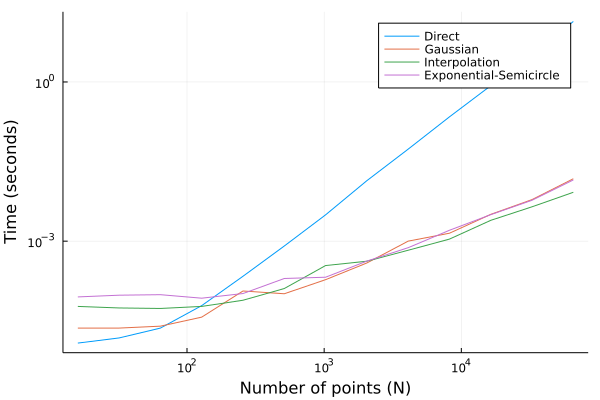
\includegraphics[width=.8\textwidth]{images/n_vs_time.png}

\end{frame}

\section{Conclusion}
\begin{frame}
  \frametitle{Conclusion}

  \begin{itemize}
      \item Sampling uniform points from nonuniform points is delicate - speed vs accuracy
      \item Selecting sampling method is an active research topic
      \item Alternative versions are appearing - low rank approximation
  \end{itemize}

\end{frame}
\end{document}
